\documentclass[12pt]{article}

% Clickable links
\usepackage[colorlinks=true,linkcolor=black,anchorcolor=black,citecolor=black,filecolor=black,menucolor=black,runcolor=black,urlcolor=black]{hyperref}

% Code blocks
\usepackage{xcolor}
\usepackage{listings}
\lstset{
	basicstyle=\ttffamily,
	showstringspaces=false,
	commentstyle=\color{red},
	keywordstyle=\color{blue},
}

% Title
\usepackage{titling}
\renewcommand\maketitlehooka{\null\mbox{}\vfill}
\renewcommand\maketitlehookd{\vfill\null}

% Section titles
\usepackage{titlesec}
\renewcommand\thesection{\Roman{section}}
\renewcommand\thesubsection{\thesection.\Roman{subsection}}
\titleformat{\section}[block]{\Large\bfseries\filcenter}{\thesection.}{1em}{}
\titleformat{\subsection}[block]{\bfseries}{\thesubsection}{1em}{}
\titleformat{\subsubsection}[hang]{\bfseries}{}{1em}{}

% Alternative heading
\usepackage{titletoc}
\setcounter{tocdepth}{2}
\dottedcontents{subsection}[5.5em]{}{4.2em}{1pc}

% Images
\usepackage{graphicx}
\graphicspath{ {./img/} }

% Preamble
\setlength\parindent{0pt}
\title{Manual de Usuario}
\author{Roberto Solares}
\date{06-07-2020}

\begin{document}

\begin{titlingpage}
	\maketitle
\end{titlingpage}

\tableofcontents
\newpage

\section{Antes de empezar}

Antes de empezar, verifica que tienes instaladas las siguientes dependencias:

\begin{itemize}
	\item Git: \url{https://git-scm.com/downloads}
	\item .NET Core 3.0 \url{https://dotnet.microsoft.com/download}
\end{itemize}

Y que tienes una copia del código fuente del proyecto. Si no lo tienes puedes descargarlo corriendo el siguiente
 comando en tu consola:

\begin{lstlisting}[language=bash]
git clone https://github.com/betoSolares/filters.git
\end{lstlisting}

Ten en cuenta que si el proyecto lo intentas correr en alguna carpeta que tenga las siguientes direcciones dará error:

\begin{itemize}
	\item src/bin/Debug/netcoreapp3.0
	\item src/bin/Release/netcoreapp3.0
\end{itemize}

\section{Ejecución}

Hay tres maneras en las que puedes ejecutar el proyecto, estas son:

\begin{enumerate}
	\item Linea de comandos (recomendada).
	\item Visual Studio Code.
	\item Visual Studio IDE.
\end{enumerate}

Todas estas tienen en común las mismas dependencias, las cuales son necesarias para que el proyecto se ejecute de
 manera correcta.

\subsection{Dependencias}

\begin{itemize}
	\item AvaloniaUI \url{https://www.nuget.org/packages/Avalonia}.
	\item Citrus.Avalonia \url{https://www.nuget.org/packages/Citrus.Avalonia}.
	\item ReactiveUI \url{https://www.nuget.org/packages/reactiveui}.
	\item .NET Core standard library, esta viene con la instalación del compilador.
\end{itemize}

\subsection{Compilación}

Esta parte solo es valida si tratas de ejecutar el proyecto mediante la linea de comandos.
 Si es así en el directorio raíz del proyecto ejecuta el siguiente comando:

\begin{lstlisting}[language=bash, xleftmargin=.4\textwidth]
dotnet build
\end{lstlisting}

Verifica que el mensaje emitido diga que la compilación fue exitosa y que hay 0 advertencias y 0 errores. \\

Si al momento de ejecutarlo encuentras un error trata de ejecutar el siguiente comando

\begin{lstlisting}[language=bash,xleftmargin=.2\textwidth]
dotnet restore && dotnet build
\end{lstlisting}

\subsection{Ejecución}

\subsubsection{Linea de comandos}

Para ejecutar el proyecto primero lo debes de haber compilado, después de haber hecho eso debes de ejecutar el
 siguiente comando en el directorio raíz del proyecto:

\begin{lstlisting}[language=bash, xleftmargin=.3\textwidth]
dotnet run -p src
\end{lstlisting}

\subsubsection{Visual Studio Code}

Para esto debes dirigirte a la sección de Ejecución o Debug en la barra de actividades.

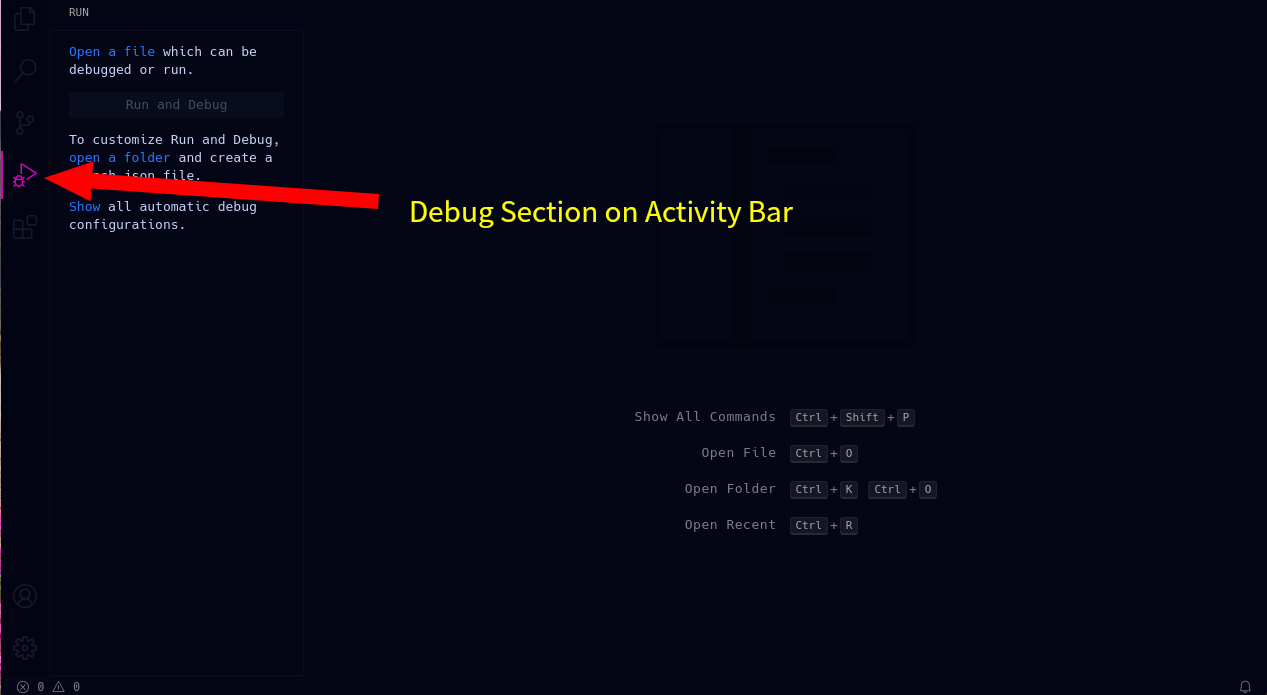
\includegraphics[width=\textwidth]{debug_section}

Luego debes hacer click al botón Run para inicializar el proyecto. \\

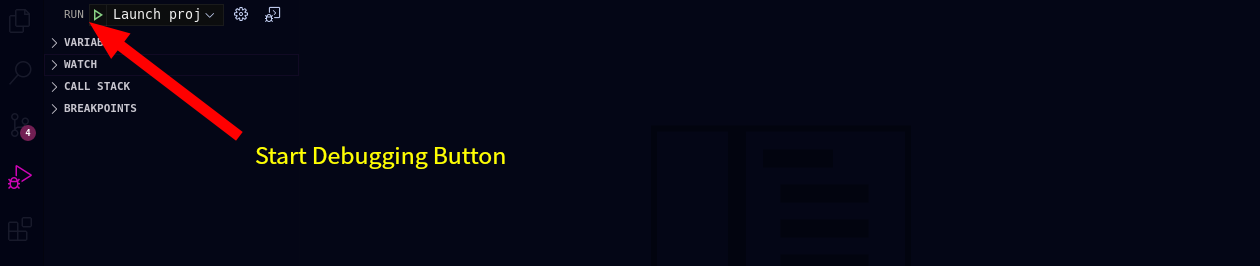
\includegraphics[width=\textwidth]{start_debugging}

Ten en cuenta que puede ser que en algunas ocasiones y dependiendo de tu sistema operativo este proceso se pueda
 demorar demasiado tiempo. Es por ello que se recomienda utilizar una terminal integrada de Visual Studio Code y
 seguir el proceso para la línea de comandos.

\subsubsection{Visual Studio IDE}

Para esta opción solo la puedes ejecutar en Windows, ya que necesitas Visual Studio IDE y este solo se puede
 ejecutar en ese sistema operativo. Aquí solo debes de darle click al botón de Start.

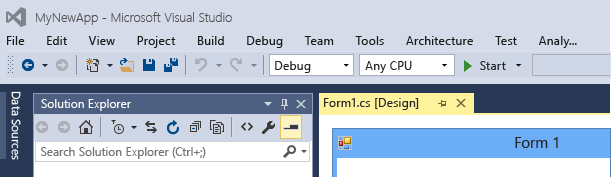
\includegraphics[width=\textwidth]{vs_ide}

\section{Explicación del proyecto}

Al momento de ejecutar el proyecto se te presentara la ventana principal del programa, esta cuenta con
 tres secciones principales las cuales son:

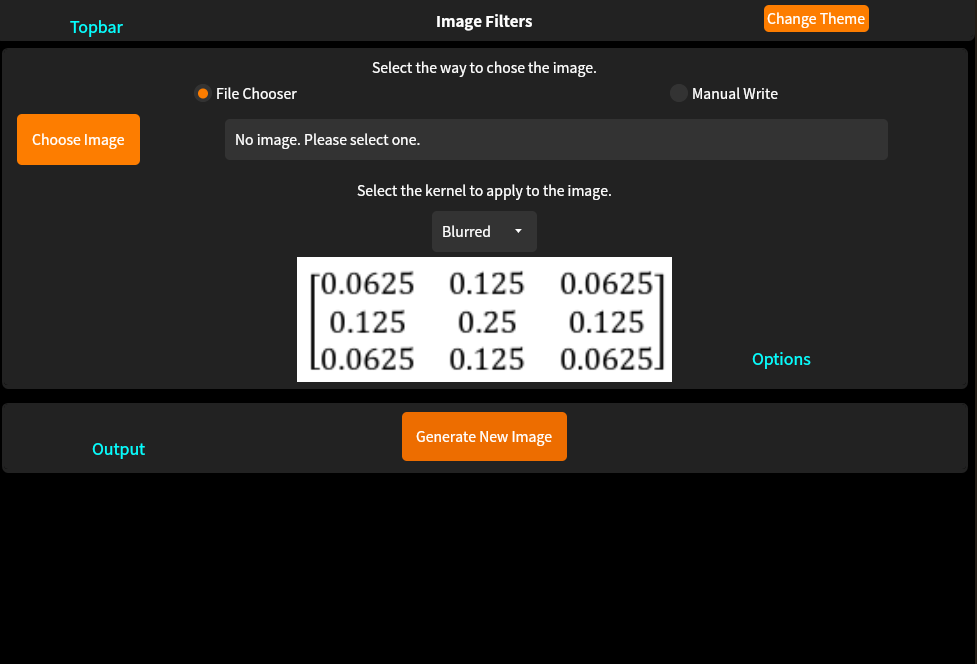
\includegraphics[width=\textwidth]{main_window}

\subsection{Topbar}

Aquí se encuentra el titulo de la aplicación y un botón con el que se puede cambiar el tema de la aplicación.

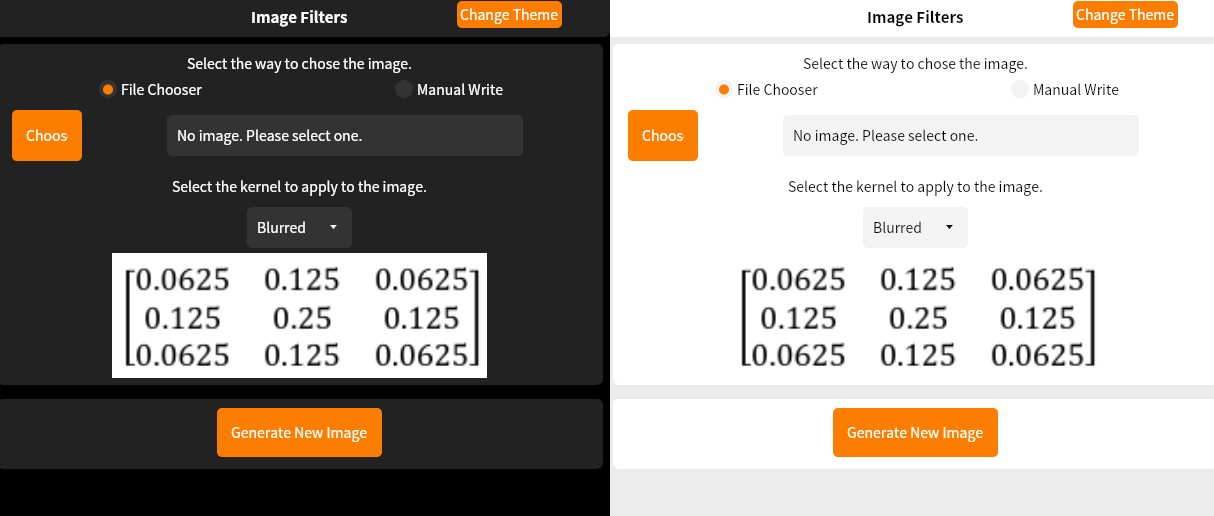
\includegraphics[width=\textwidth]{themes}

\subsection{Options}

Aquí puedes seleccionar la imagen a la que deseas aplicarle el filtro, para ello solo debes de hacer click en el
 botón Choose, es posible que si estas ejecutando la aplicación en Linux o macOS esta funcionalidad haga a la
 aplicación fallar, para ello solo debes de seleccionar el método de entrada Manual Write y después escribir la
 dirección a la imagen de manera manual en el textbox. \\

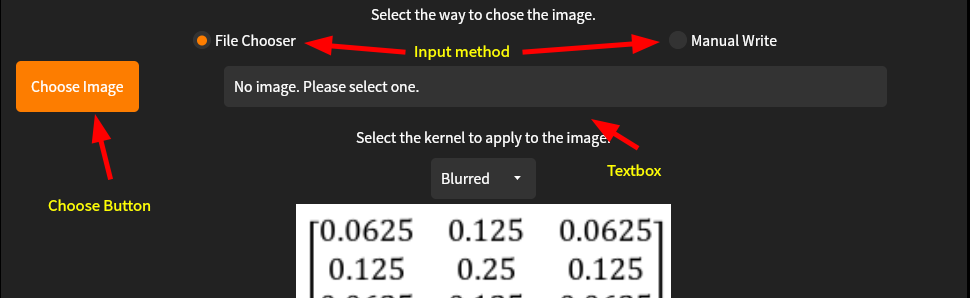
\includegraphics[width=\textwidth]{image_selection}

Después tienes la opción de seleccionar varios filtros que se le pueden ser aplicados a la imagen, si seleccionas
 la opción Custom te aparecerá una tabla en la que podrás ingresar los valores para cada una de las posiciones
 que se te pide, ten en cuenta que en esta solo podrás ingresar números y cualquier letras que ingreses sera
 descartada. \\

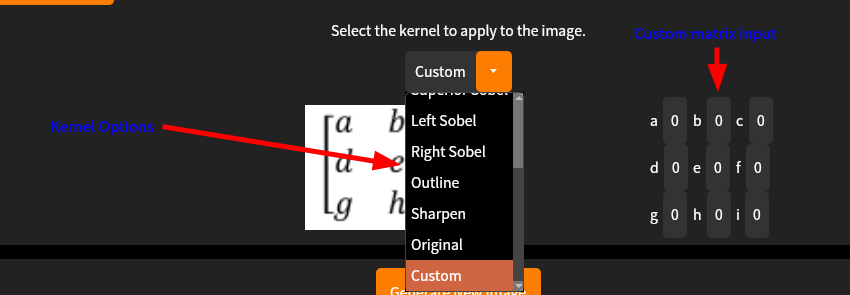
\includegraphics[width=\textwidth]{kernel_selection}

\subsection{Output}

Después de que has seleccionado la imagen y el kernel que se le aplicara, debes de darle click al botón de Generate
 New Image, el cual aplicara el algoritmo de filtrado a la imagen. Las matrices que se utilizan para cada filtro
 son las siguientes: \\

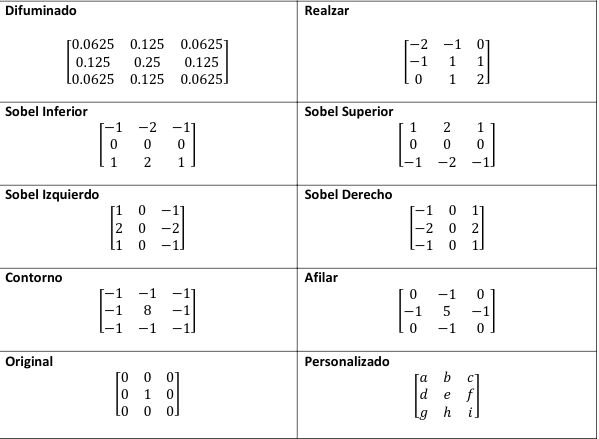
\includegraphics[width=\textwidth]{kernels}

Con la única diferencia de que para el filtro Blur se utiliza la matriz no normalizada, ya que para esta es mucho
 mas fácil aplicar el algoritmo al no tener que balancear los pesos de la matriz. Para resolver el problema de los
 bordes en cada filtro se utilizo el algoritmo de Extensión, el cual utiliza los pixeles mas cercanos y los
 extiende tanto como sea necesario. Los pixeles se extienden en lineas rectas. \\

Luego de que se ha generado la imagen veras los resultados de todo el proceso así como un mensaje indicando en donde
 han sido guardadas las imágenes. \\

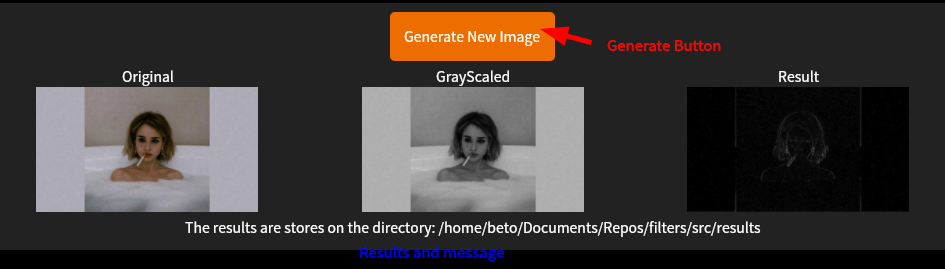
\includegraphics[width=\textwidth]{results}

\end{document}
